\documentclass[11pt]{ltjarticle}
\usepackage[b5paper,bmargin=100pt]{geometry}
\usepackage{luatexja}
\usepackage[utf8]{inputenc}
\usepackage{amsmath}
\usepackage{amssymb}
\usepackage{mathtools}
\usepackage{musicography}
\usepackage{leadsheets}
\usepackage{luatexja-ruby} 
\usepackage{wrapfig}
\usepackage{caption}
\usepackage{makecell}
\usepackage{dashrule}
\usepackage{graphicx}
\usepackage{xcolor}
\graphicspath{ {./resources/} }
\usepackage{hyperref}
\usepackage{subcaption}
\usepackage[document]{ragged2e}

\setchords{
    major-seven = \textsuperscript{M7},
    major-nine = \textsuperscript{M9}
}

\renewcommand*\contentsname{目次}
\renewcommand{\figureautorefname}{図}
\renewcommand{\tableautorefname}{表}
\setlength{\RaggedRightParindent}{\parindent}
\setlength{\abovecaptionskip}{0pt plus 3pt minus 2pt}
\RaggedRight
%\pagenumbering{roman}
\pagenumbering{gobble}
\addtocounter{page}{1}
\setcounter{tocdepth}{2}

%\title{コードオタクが語る東方楽曲分析 \\ \large{第二弾　緋想天 - 砕月からみるメロディーの作り方}}
\author{Metalloid.}
\date{Oct 2025}

\newcommand{\wc}{\writechord}
%\newcommand{\sd}{\textbf}
\NewDocumentCommand{\sd}{}{\musDegree}


\begin{document}
%\maketitle

\Center{\huge{試作 Golden Land}}
\vspace{3pt}
\hrule
\vspace{3pt}
\rightline{\large{原曲：プレステ・ジョアンの黄金境 }}
\vspace{12pt} \rightline{作曲：上海アリス幻樂団} \rightline{編曲：Metalloid.}

%\tableofcontents

\vspace{7pt}

\begin{figure}[h]
    \centering
    
\includegraphics[width=0.38\linewidth]{qr song.png}
\end{figure}
\vspace{-10pt}
\section*{アレンジャーコメント}
\RaggedRight
錦上京フィーバー（＆七弦ギター個人的フィーバー）の時期に色々試してできた試作ですが、このままこれ以上進展させることが難しそうだったので、供養という形で出してみることにしました。今回の着眼点としては、錦上京曲と遊びつつ、ギターを録音せずに音源ギターを用いてどこまでそれっぽく聞こえさせられるかの二点です。\par
前半は速めのテンポを刻みながら、どこか切ない、綺麗なコード感を展開しようとしたものです。特に書いていて気に入ったのはイントロ？間奏？のような箇所で、上下リードギター、上下シンセが移り変わるバックのコード進行に対して同じパターンをハモリながら繰り返すところですね。裏打ちのハイハットに聞こえるシンセも実はドラムではなく同じシンセが裏拍だけ高音に逃げている音で、コードに対してエモめの音を鳴らすことによって切なさを出しているといった感じです。\par 
後半は、和音がかなり動く前半とは真逆の解釈を実践してみたところで、ギター・ベース・ドラムから成るリズム隊の奏でるリズム的美学を楽しむことができる脱和声的なセクションが主眼です。その後ちょっとしたピアノ休憩を経てから、脱和声セクションに壮大重厚なハモリを追加し、バックのコード進行を動かすことによって抜けていた和声を回帰させ、サビっぽいもの（？）を登場させています。ここでもリズム的美学が主眼といいつつも、二回し目でちょっとした不協和音をギターに混在させて和声美を仄めかしております。と云いたいところですが、恐らく手癖を入れたい欲望に耐えきれなくなっただけなのでしょう。\par
その後再び前半の気に入りフレーズで曲を終わらせていますが、実はキーが最初と最後でズレてしまったがために、ギターチューニングの関係でちょっとギターのハモり方が異なります。聞こえないけど。
\begin{figure}[h]
    \centering
    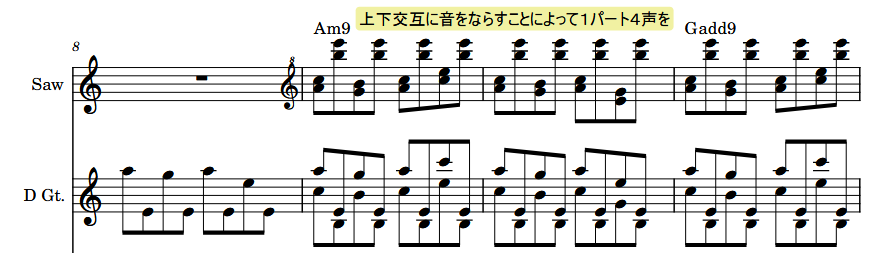
\includegraphics[width=0.9\linewidth]{snippet.png}
    \label{fig:snippet}
    \caption{前半のイントロ？間奏？の旋律楽器抜粋}
\end{figure}
\end{document}
